%************************************************
\chapter[Interactions and environmental factors]{Community responses to resource and non-resource environmental gradients}\label{ch:environment}
%************************************************

%\tikz[remember picture,overlay] \node[opacity=0.3,inner sep=0pt] at (current page.center){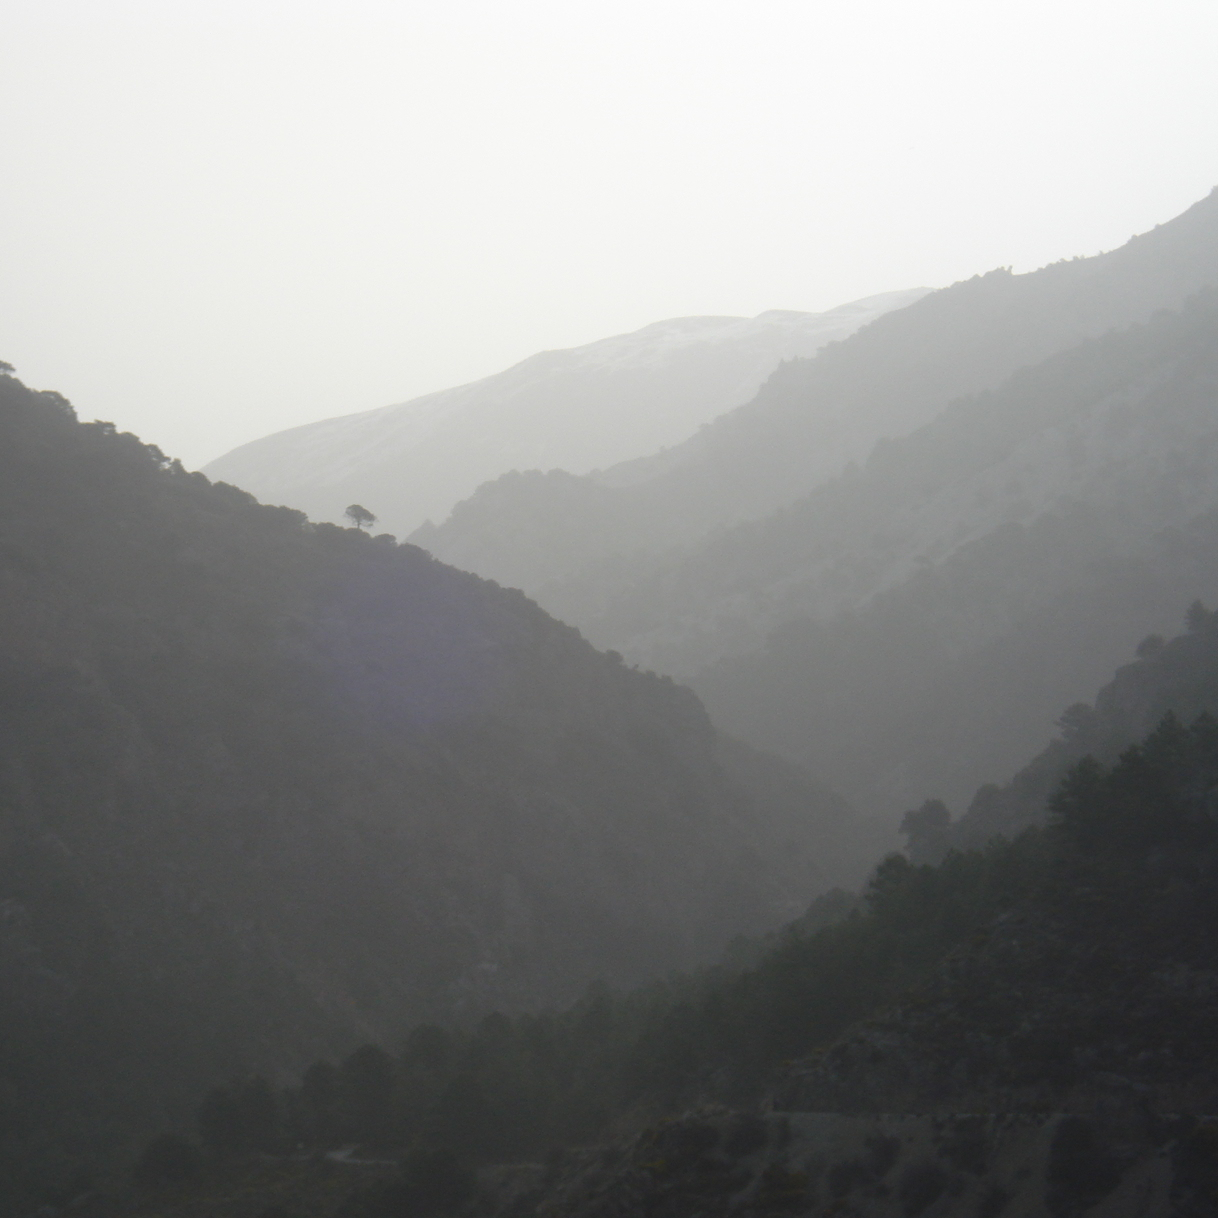
\includegraphics[width=\paperwidth,height=\paperheight]{./Figures/cover/granada_2_pagina.jpg}};
\tikz[remember picture,overlay] \node[opacity=0.3,inner sep=0pt] at ([yshift=3cm,xshift=2cm]current page.center){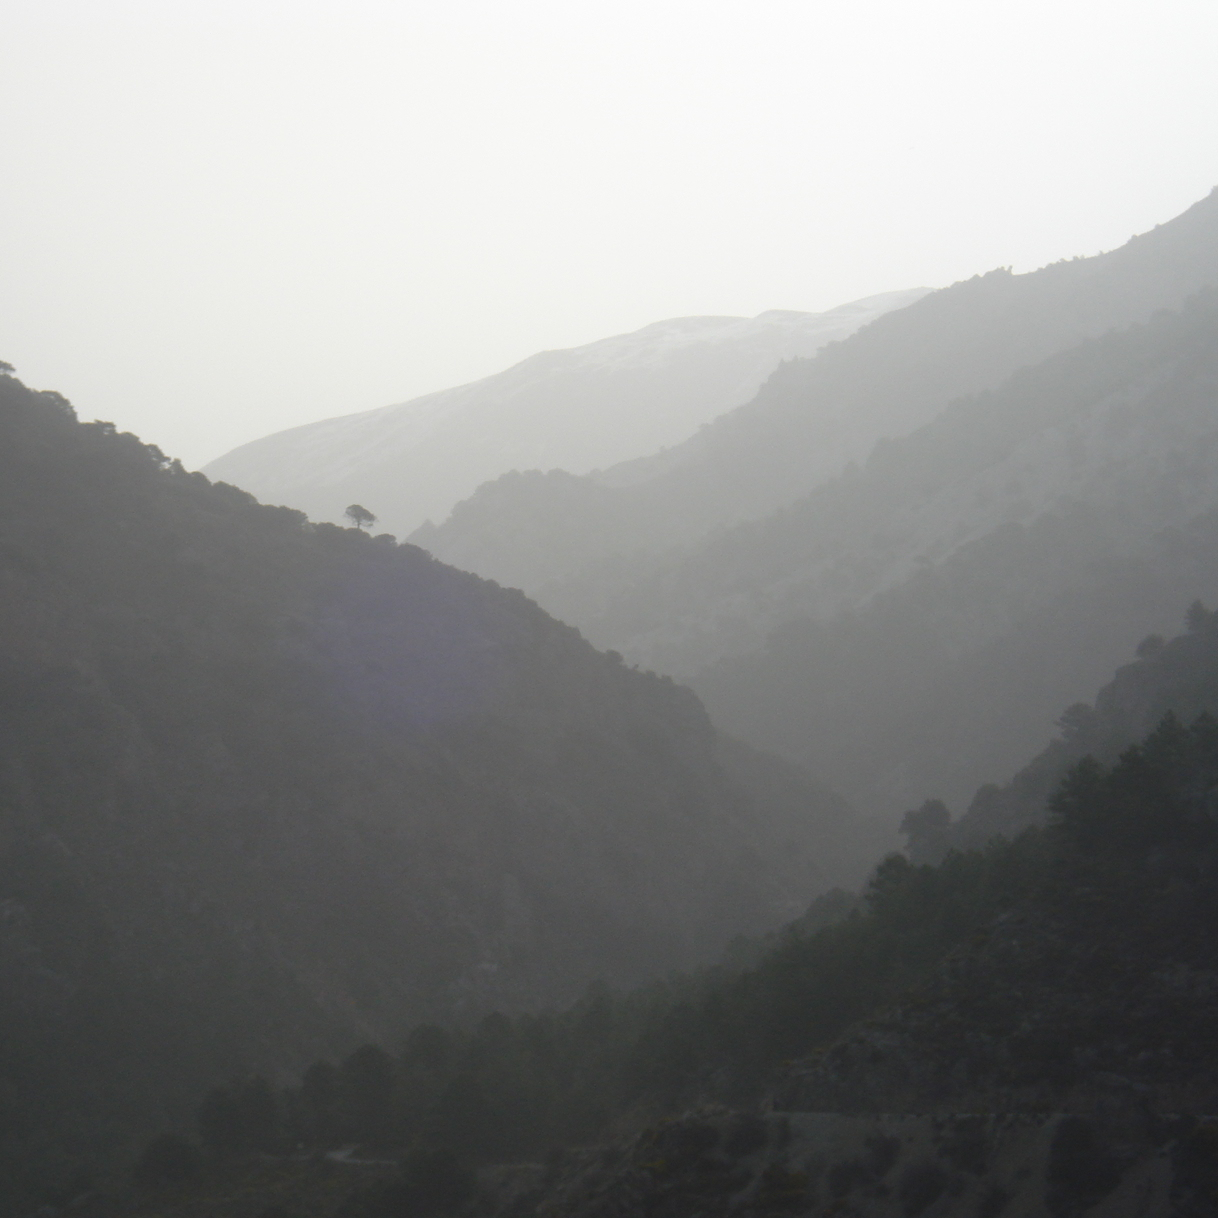
\includegraphics[width=\paperwidth,height=\paperheight]{./Figures/cover/granada_2_pagina.jpg}};
\clearpage

\section*{Abstract}

Environmental variations are a driving force behind virtually all ecological patterns. Different types of environmental gradients are bound to trigger differential responses at the species and community level, but this variability among environmental factors has been largely overlooked in current community ecology paradigms. We argue that the distinction between resource and non-resource factors, originally proposed by Evelyn G. Hutchinson, provides a convenient way to classify environmental factors, as these two types have different effects on ecological interactions and emergent community properties. Using a community model with environmental variability on a resource and a non-resource factor, we show that the intensity of competitive interactions is driven jointly by variations in both gradients, whereas facilitation intensity is driven solely by the non-resource factor. Likewise, species richness and persistence times of species are mainly driven by variations in the non-resource factor. These results, derived for simple model communities, suggest the possibility that these two broad types of environmental gradients trigger different bottom-up and top-down feedbacks in more complex communities.

\section{Introduction}

Understanding how environmental factors influence ecological processes is one of the main goals of ecology, and is becoming increasingly relevant in the context of the ongoing global change \citep{Vitousek1994}. Environmental factors influence directly or indirectly virtually every biological process on Earth, and can be extremely varied in their physical characteristics, magnitude, spatial and temporal scale. Furthermore, individuals may interact and respond to their physical environment in very different ways: sessile primary producers acquire inorganic nutrients from their surrounding environment and can often modify their local microclimate, whereas animals are able to move or alter their behaviour in response to environmental variations. Despite the enormous variability in environmental variables and species responses, different environmental factors are commonly lumped together when studying ecological processes across observed gradients, in what are termed “(environmental) stress gradients” (e.g. \citealt{Hart2013}).

As a consequence of this common simplification of environmental factors, there is no overarching theory predicting how different facets of the environment will influence ecological processes at different levels of organization. Developing, or as we will suggest here, recovering a simple but comprehensive “taxonomy” of environmental factors is a key step towards such a theory. To our knowledge, only a handful of studies have attempted to derive a systematic characterization of environmental factors. For example, \cite{Menge1987} made the distinction between physical and physiological stress types, that differ on whether low values of the factor at hand influence survival. Although their classification is readily applicable to any species and gradient, it is not informative about which factors may drive variations in pairwise interactions or resource consumption, which are key processes for maintaining species coexistence.

In the context of niche theory, Evelyn G. \cite{Hutchinson1978} proposed the distinction between scenopoetic and bionomic variables that shape the n-dimensional environmental niche of a given species. Scenopoetic variables are, literally, “scene-setting” factors, abiotic conditions that cannot be consumed, whereas bionomic variables are those consumed by the species or guild in question, thus altering their local dynamics. This distinction has been acknowledged, with a different terminology, in studies of vegetation composition across gradients \citep{Austin1990}. In addition, the stress gradient hypothesis, in its general form, posits that variations in stress levels will drive variations in the intensity of competitive and facilitative interactions among primary producers, with positive interactions becoming more prevalent under harsh conditions \citep{Bertness1994}. A few studies have explored how this hypothesis might be improved by distinguishing resource (i.e. bionomic) and non-resource (scenopoetic) environmental factors. For example, a recent study suggested varying outcomes of pairwise interactions under gradients of different types of factors \citep{Maestre2009}, whereas a compilation of empirical data showed similar shifts towards facilitative interactions across gradients of different stress types \citep{He2013}. Despite these recent developments, most empirical tests of the stress gradient hypothesis do not explicitly consider the implications of studying resource, non-resource, or combined gradients. Furthermore, this diversity of factors has thus far been left out of other influential frameworks in community ecology, such as Tilman’s resource ratio theory \citep{Tilman1980, Miller2005}, environmental stress models \citep{Menge1987}, or Chesson’s coexistence theory \citep{Chesson2000}.

We propose to reintegrate the fundamental distinction between environmental factors coined by \cite{Hutchinson1978} into current ecological paradigms. Hutchinson’s categorisation provides a simple dichotomy for environmental factor types that is relevant for evaluating physiological responses, and most importantly, the outcome of direct pairwise interactions and other community-level responses to environmental gradients. Maintaining the terminology that has recently been developed under the umbrella of the stress gradient theory, we propose to keep the name of resource and non-resource environmental factors for bionomic and scenopoetic variables respectively (Fig. \ref{fig:fig6.1}).

While at the individual level most species will display varying physiological response curves for specific factors regardless of their resource or non-resource quality, the distinction between these categories becomes important when looking at the differences of these response curves between species. As such, we may expect responses to resource factors to be nested for groups of species, while responses to non-resource factors will likely tend to have different optima for different species of a guild \citep{Austin1990}.

Looking at community-level responses, we hypothesize that variation in resource factors will directly drive exploitative competition within species of the same trophic guild, whereas variation in non-resource factors will, instead, drive changes in the intensity and importance of facilitation, and only indirectly will affect competition. These pairwise effects will, in turn, drive different outcomes for species persistence or diversity, among other properties, across different types of gradients.

Here we test these hypotheses using a community model in which we incorporate gradients of resource and non-resource environmental factors. In particular, we ask: (1) does the intensity of competitive and facilitative interactions vary across a combined resource and non-resource environmental gradient? (2) how are species diversity and persistence affected by environmental variation? (3) does the presence of benefactor species increase species diversity and persistence in our model communities? In the following sections, we briefly expand on the two types of environmental factors proposed, and then we discuss our modelling experiment.

\subsection{Non-resource environmental factors}

Non-resource factors are the scenopoetic variables of \cite{Hutchinson1978}, not consumed by individuals, and thus not subjected to depletion. These factors have a direct physiological impact on all individuals, and many of them are expected to have broad spatial structures \citep{Soberon2007}. Response curves may show different optima for different species, and are unimodal \citep{Austin1990}. There are two main ways in which species can alter these factors: first, sessile species may passively generate microhabitats with different conditions from those of the surrounding area. Second, some mobile species are considered ecosystem engineers, species that actively modify their surrounding physical environment thus generating different conditions.

By varying their surrounding environment, sessile species and ecosystem engineers generate environmental conditions that allow the establishment of other individuals that would not be able to thrive otherwise. Thus, facilitative interactions are commonly found to increase in intensity with increasing stress from non-resource factors such as temperature or wind exposure (e.g. \citealt{Fajardo2011}). By definition, as these factors are not subject to consumption, non-resource gradients will not directly drive variations in competition intensity (although by excluding less adapted individuals, overall competition intensity is often reduced in sites with high non-resource stress).

\subsection{Resource environmental factors}

This category includes all factors that are consumed by the species or guild under study. When referring to terrestrial plants, the set of resources is limited to light and space, water, carbon dioxide, oxygen, and essential nutrients \citep{Austin1990}. Each of these resources, in turn, has different spatiotemporal dynamics. Conceptually, feeding sources of consumer species may be considered as resource factors, but these resources are highly dynamic and consumers are often able to switch between different preys, whereas abiotic resources are generally not interchangeable.

Gradients in resource factors will drive variations in exploitative competition when different individuals utilise the same resource. On the other hand, these factors are generally not subject to facilitation, and therefore, the intensity of pairwise facilitation should in general not vary when the only source of environmental variation is a resource factor. As discussed in \cite{Maestre2009}, the case of water availability is more complex than this baseline expectation, as water availability is highly correlated with temperature levels, and may be subject to facilitation under some circumstances (see Discussion).

\begin{figure}[ht]
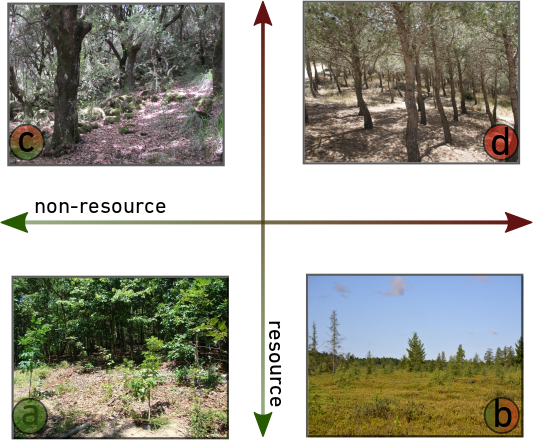
\includegraphics[width=\textwidth]{./Figures/chapter06/Fig_1.png}
\caption[Resource and non-resource environmental gradients]{\color{Gray} A two dimensional environmental gradient. In this example, the non-resource factor  is soil ph, and the resource factor is available direct sunlight. Considering a plant species with optimal fitness at basic ph levels and high levels of direct sunlight, the environmental gradients show different combinations of factors: (a) suitable light and ph levels may be found in open areas or forest gaps on basic soils, (b) peat bogs are highly acidic environments, but otherwise suitable regarding light levels, (c) closed canopies under basic soils may have too low light levels, (d) understoreys of pine forests have both low light levels and acidic soils.}
\label{fig:fig6.1}
\end{figure}

\section{Methods}

\subsection*{Modelling community responses to a combined gradient}

The basic tenets presented above apply, all else being equal, to gradients of only one factor at a time. However, it is harder to derive conceptual predictions about variations across combined gradients of both types. Using a simple community model, we analysed whether variations in two environmental factors, a resource and a non-resource one, drive variations in different patterns of a horizontal community (composed of a single trophic guild). We generated a pool of species with varying demographic responses to non-resource stress factors, following the functional responses discussed in \cite{Maestre2009}, in which species vary their survival and growth rates according to the level of non-resource stress (Appendix 6.1). The two extreme cases in this framework are, on the one hand, stress-tolerant species, that are able to maintain comparatively high survival rates under high stress levels, but display lower growth rates in the absence of stress; and competitive species on the other hand, that show high growth rates under benign conditions but also higher sensitivity in both survival and growth rates to non-resource stress.

In our model setting, environmental variability is represented by a two-dimensional lattice, in which each cell has a combination of resource and non-resource environmental factors (Appendix A.6.1: Figure A.6.1.1). The resource factor is represented as the carrying capacity of the cell, and all species are assumed to belong to the same trophic guild (sensu \citealt{Fauth1996}), whose only limiting factor is that resource. The non-resource factor is homogeneous and constant in a given cell. Both gradients are linear.

Species randomly colonize with equal probability any given cell of the lattice, and survive and grow according to their specific functional responses (Appendix A.6.1: Figure A.6.1.2). A fraction of species is able to facilitate the survival of heterospecifics, by enhancing their survival probability in the face of high levels of non-resource stress. The intensity of each facilitation event is given by the biomass of the benefited individual, that would have otherwise not survived.

Individuals in a cell are able to grow up to the level where their aggregated biomass equals the carrying capacity of the cell, i.e. the level of resource factor. Competition occurs when the growth of one or more individuals is hampered due to the presence of another individual, and its intensity is given by the amount of expected growth that was impeded by the competitive exclusion.

With this simple setting, we modelled how species interact and persist through time in each combination of the two gradients. After an initial warm-up period of 100 timesteps, to allow each cell to be colonised, we recorded for 500 timesteps every facilitative and competitive interaction, the effective number of species at each cell (also known as “Hill number” or “true diversity”, \citealt{Tuomisto2012}), and the average persistence time of species at each cell. To evaluate the response of these metrics to the environmental gradients, we fitted generalised additive models (GAMs) to the results from our simulations. Generalised additive models use smoothing functions to model nonlinear relationships, providing a flexible nonparametric model \citep{Wood2017}. Given the strong nonlinearities observed in our responses, we fitted GAMs with adaptive smoothing terms, that are able to model responses where the degree of smoothness vary over the range of the covariates \citep{Wood2017}.

We also performed simulations with the same parameterization but not allowing for facilitation, and compared the distributions of competition intensity, species diversity, and persistence times in the two sets of simulations, using Wilcoxon signed-rank tests.

\section{Results}

\subsection*{Does the intensity of competitive and facilitative interactions vary across a combined resource and non-resource environmental gradient?}

The intensity of competition and facilitation strongly varies across the combined environmental gradient (Fig. \ref{fig:fig6.2}, Table \ref{tab:tab6.1}). Competition intensity increases with increasing resource stress (Fig. \ref{fig:fig6.2}, panel a) and with decreasing non-resource stress (Fig. \ref{fig:fig6.2}, panel b), and the interaction between resource and non-resource stress is also statistically significant (Table \ref{tab:tab6.1}). Facilitation intensity, in turn, is only significantly influenced by non-resource stress (Table \ref{tab:tab6.1}, Fig. \ref{fig:fig6.2}, panel c and d). In absence of stress, there is no facilitation, as every species has a survival probability of 1 (Appendix A.6.1: Figure A.6.1.2). Then, as non-resource stress increases, facilitation intensity displays a concave parabolic shape: it is high and very variable for low levels of stress, lowest for intermediate levels, and consistently high and comparatively less variable for high stress levels.

\clearpage
\begin{landscape}
\begin{table}[] \footnotesize
\caption[GAM model results]{\color{Gray}Results of the Generalised Additive Models fitted to the simulation results. REML = Restricted maximum likelihood. For parametric coefficients, their estimates, standard errors, and t-statistic are given, whereas for smooth terms, we report their estimated degrees of freedom (edf), and their F-statistic.}\label{tab:tab6.1}
\begin{tabular}{lllllllllll}
\hline
Response                                                                               & REML                     & $r^{2}$ & Deviance                & Covariates               & Estimate  & Std.Error  & t      & edf   & F      & p-value        \\
\hline
\multirow{3}{*}{\begin{tabular}[c]{@{}l@{}}facilitation\\ intensity\end{tabular}}      & \multirow{3}{*}{-1376.2} & \multirow{3}{*}{0.528}   & \multirow{3}{*}{53.1\%} & intercept                & 0.674     & $6.3*10^{-3}$ & 106.56 & -     & -      & $< 0.05$ \\
                                                                                       &                          &                          &                         & resource                 & $-4.8*10^{-5}$ & $1*10^{-4}$     & -0.465 & -     & -      & 0.642          \\
                                                                                       &                          &                          &                         & s(non-resource)          & -         & -          & -      & 14.16 & 167.5  & $< 0.05$ \\
\multirow{4}{*}{\begin{tabular}[c]{@{}l@{}}competition\\ intensity\end{tabular}}       & \multirow{4}{*}{-5459.3} & \multirow{4}{*}{0.967}   & \multirow{4}{*}{96.7\%} & intercept                & 0.108     & $5.2*10^{-4}$   & 208.4  & -     & -      & $< 0.05$ \\
                                                                                       &                          &                          &                         & s(resource)              & -         & -          & -      & 3.28  & 7405   & $< 0.05$ \\
                                                                                       &                          &                          &                         & s(non-resource)          & -         & -          & -      & 12.53 & 1813.5 & $< 0.05$ \\
                                                                                       &                          &                          &                         & s(resource*non-resource) & -         & -          & -      & 25    & 262.4  & $< 0.05$ \\
\multirow{3}{*}{\begin{tabular}[c]{@{}l@{}}persistence\\ times\end{tabular}}                                                     & \multirow{3}{*}{7451.8}  & \multirow{3}{*}{0.986}   & \multirow{3}{*}{98.6\%} & intercept                & 26.18     & 0.217      & 120.71 & -     & -      & $< 0.05$ \\
                                                                                       &                          &                          &                         & resource                 & $2.2*10^{-3}$  & $3.5*10^{-3}$   & -0.625 & -     & -      & 0.532          \\
                                                                                       &                          &                          &                         & s(non-resource)          & -         & -          & -      & 14.29 & 10741  & $< 0.05$ \\
\multirow{3}{*}{\begin{tabular}[c]{@{}l@{}}effective\\ richness\end{tabular}} & \multirow{3}{*}{4127.2}  & \multirow{3}{*}{0.922}   & \multirow{3}{*}{92.2\%} & intercept                & 4.828     & 0.057      & 83.92  & -     & -      & $< 0.05$ \\
                                                                                       &                          &                          &                         & resource                 & -0.016    & $9.4*10^{-4}$   & -16.64 & -     & -      & $< 0.05$ \\
                                                                                       &                          &                          &                         & s(non-resource)          & -         & -          & -      & 10.36 & 2355   & $< 0.05$
%\hline
\end{tabular}

\end{table}

\begin{table}[]
\caption[Facilitation impacts]{\color{Gray}Results of the Wilcoxon signed-rank tests for differences in competition intensity, species diversity, and average persistence times between communities with and without facilitation. Test on competition intensity is two-tailed, reflecting our lack of previous hypotheses on the intensity of competitive effects between the two sets of simulations. Tests on species diversity and persistence are one-tailed, with the alternative hypothesis being greater values of both metrics when facilitation is allowed. In bold, highest median values of each quantity.}\label{tab:tab6.2}
\begin{tabular}{lllll}
\hline
 & median - facilitation & median - no facilitation & V & p-value \\
\hline
\begin{tabular}[c]{@{}l@{}}competition\\ intensity\end{tabular} & \textbf{0.059} & 0.050 & 1229233 & $< 0.05$ \\
persistence times & \textbf{15.47} & 12.369 & 2401500 & $< 0.05$ \\
effective richness & \textbf{2.374} & 2.067 & 2600200 & $< 0.05$
%\hline
\end{tabular}

\end{table}

\end{landscape}

\subsection*{How are species diversity and persistence affected by the environmental variation?}

The effective number of species at each cell drops rapidly with even slight increases in non-resource stress (Fig. \ref{fig:fig6.2}, panel f), and also shows a decreasing trend, although less steep, with increasing resource stress (Fig. \ref{fig:fig6.2}, panel e). Average persistence time, in turn, also decreases very sharply with non-resource stress (Fig. \ref{fig:fig6.2}, panel h), but is unaffected by resource stress (table \ref{tab:tab6.1}, Fig. \ref{fig:fig6.2}, panel g).

\subsection*{Does the presence of benefactor species increase species diversity and persistence in our model communities?}

Both species diversity and persistence times are significantly higher in simulations with facilitation (Table \ref{tab:tab6.2}, Appendix A.6.1: Figure A.6.1.4).

\begin{figure}[ht]
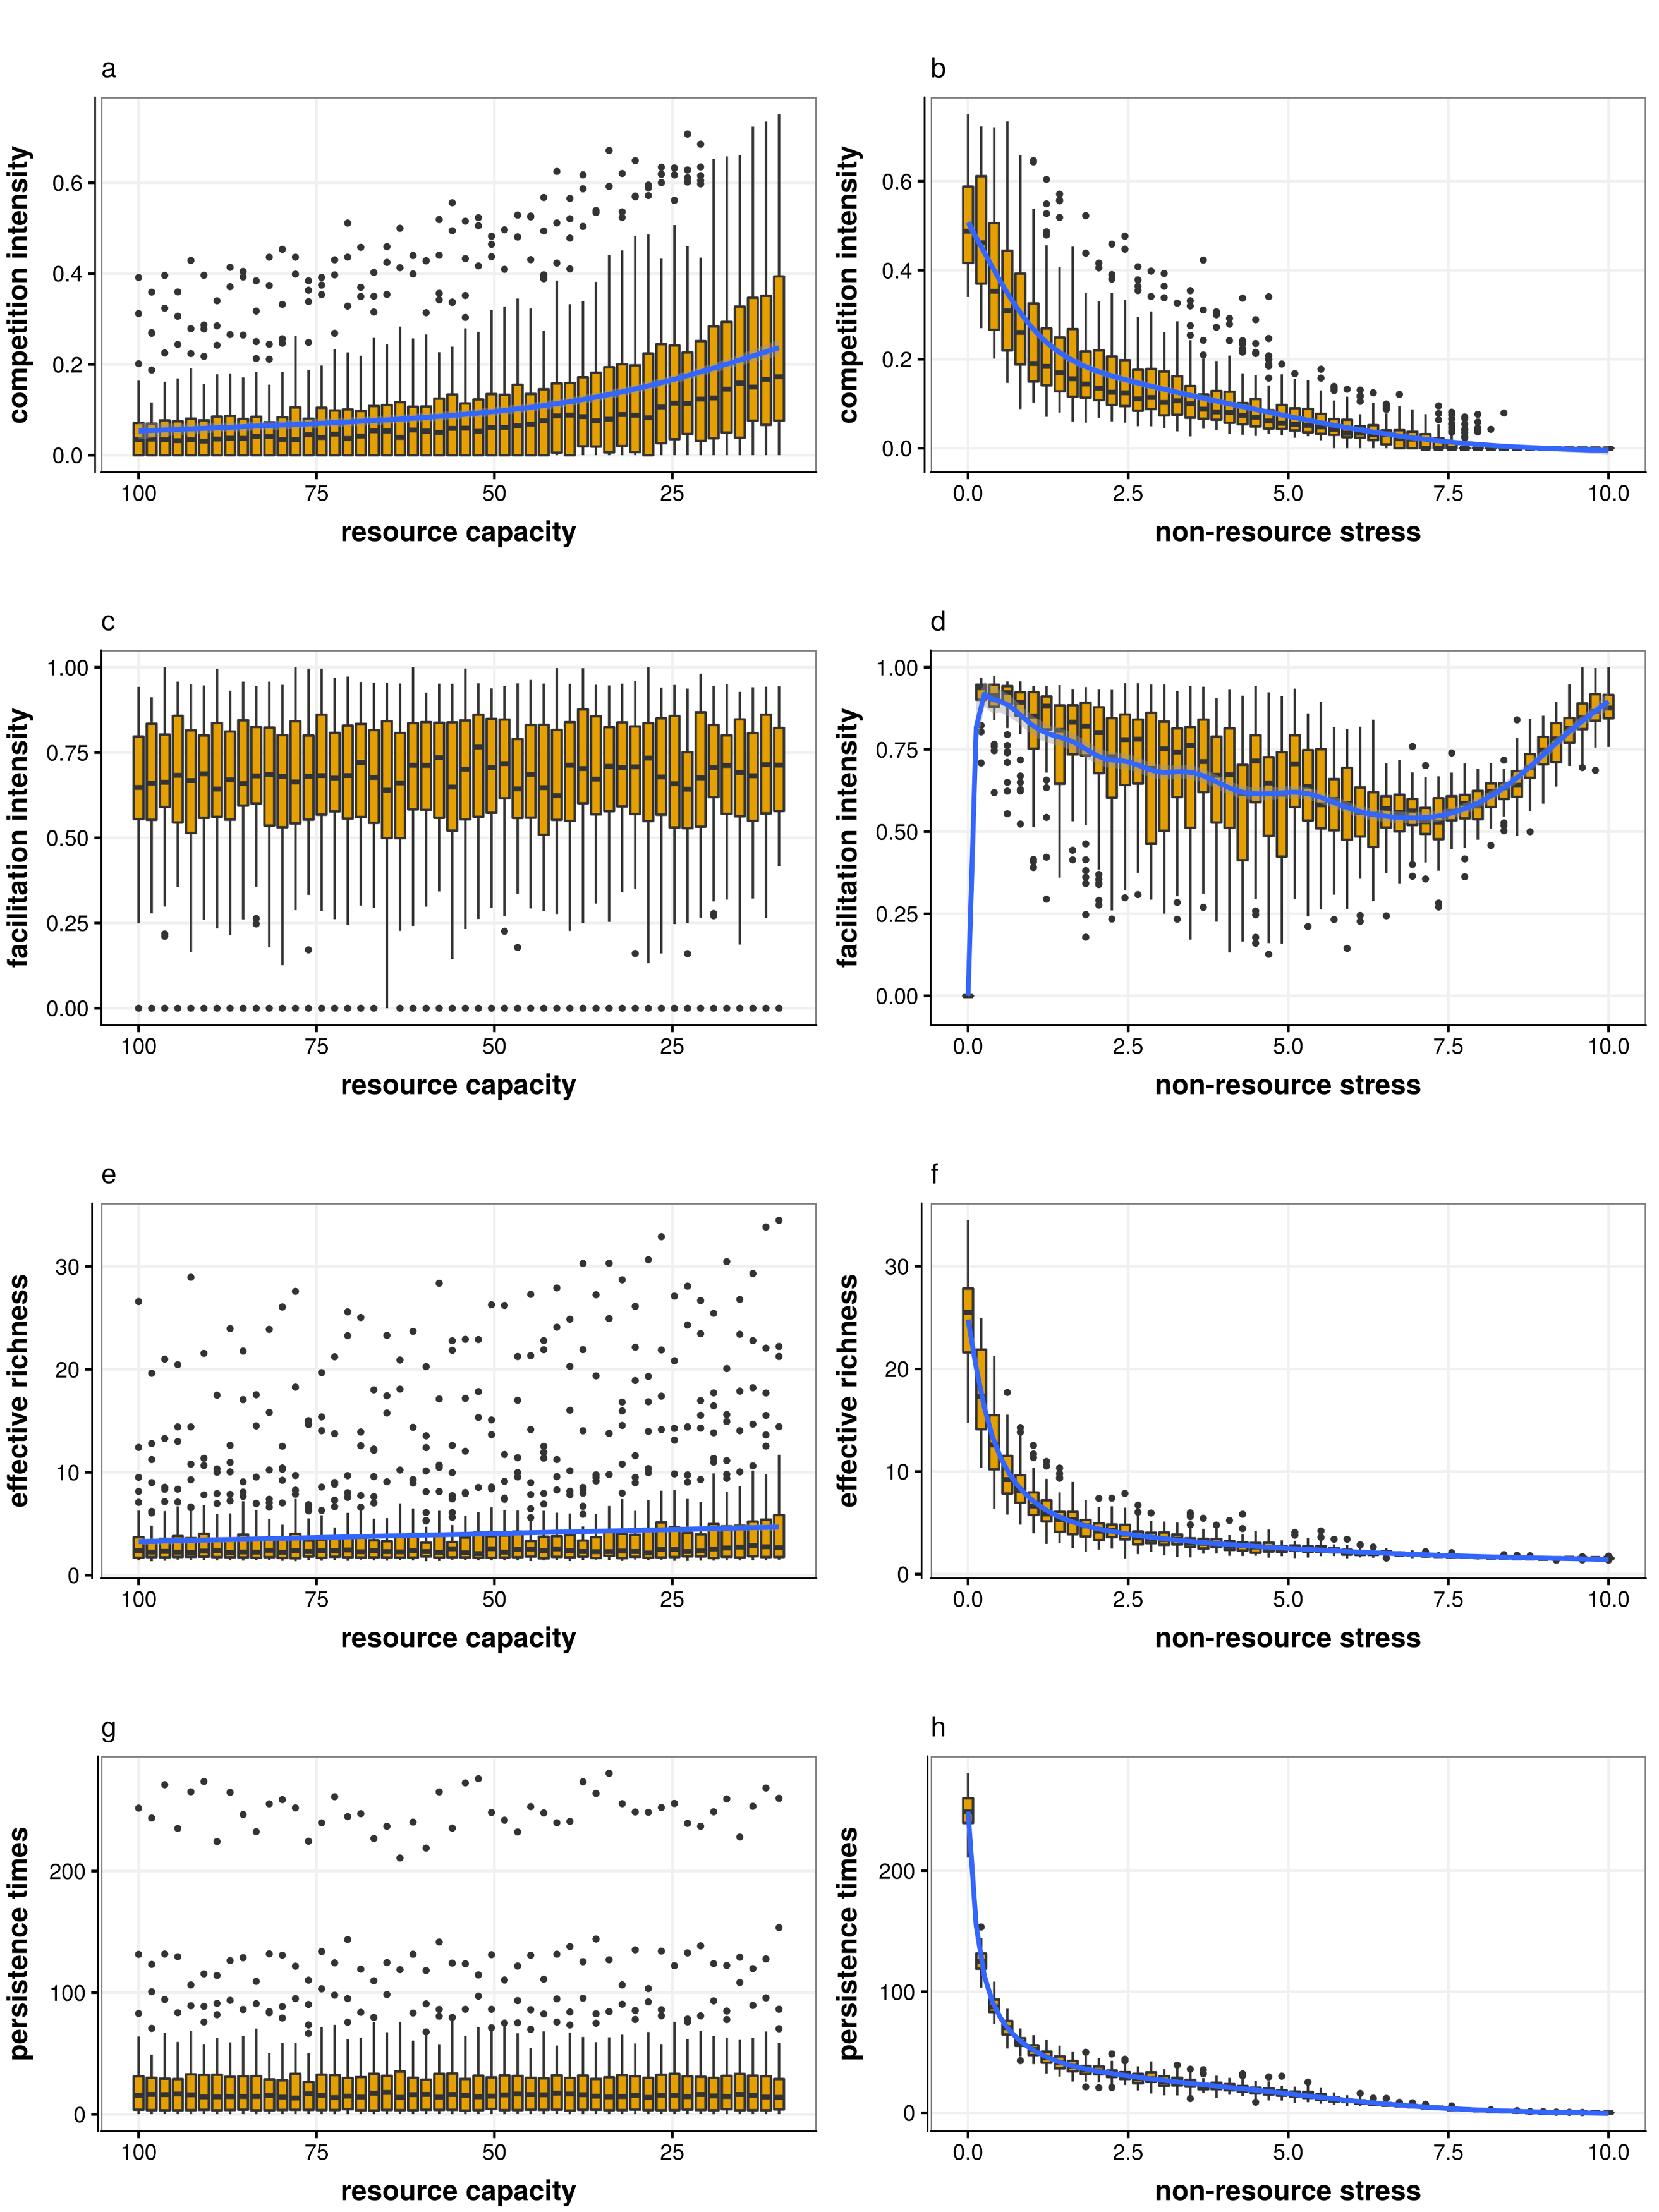
\includegraphics[width=\textwidth]{./Figures/chapter06/Fig_2.png}
\caption[Community responses to gradients]{\color{Gray} Variation of community-level properties across a resource and a non-resource gradient. For variables selected as significant by the GAM models (Table \ref{tab:tab6.1}), model fits are superimposed as blue curves.}
\label{fig:fig6.2}
\end{figure}

\section{Discussion}

We modelled the response of species ranging from pure competitors to pure stress-tolerance within a two-dimensional environmental gradient combining a resource and non-resource factor. The two types of environmental factors have contrasting influences on (1) the intensity of pairwise interactions and (2) the diversity of species in the community and their average persistence times.

The intensity of competitive interactions clearly increases with increasing levels of resource stress, as expected. However, it also increases for decreasing levels of non-resource stress. This is due to the positive correlation observed between mortality rates and non-resource stress, that releases resources and decreases effective competition at highly stressful environments.

Facilitation is, again as we hypothesised, clearly driven by variations in the non-resource factor. The response observed is, however, more complex than the standard expectations derived from the stress-gradient hypothesis, that predicts either an increasing importance of facilitation with increasing stress, or an increase followed by a collapse in facilitation levels at very high stress levels \citep{leRoux2010}. The idea behind this latter version of the theory is that in extremely harsh environments, the facilitation effect of nurse plants is severely hampered \citep{Michalet2006}. This reasoning, however, only applies to non-resource factors, as species do not compete for them; if the environmental gradient includes resource factors, net interaction effect may switch from positive to neutral or negative \citep{Smit2007,Michalet2014}. In our simulations, we first observed, as expected, no facilitation in the absence of non-resource stress. As soon as there is a certain environmental impact on competitive species, however, facilitation sharply increases, while at the same time showing a high variability. We argue that this unexpected variability is due to priority effects, in which the order of arrival of species to a location is an important factor for the subsequent dynamics of the local community \citep{Fukami2015}. In our model, all species have the same probability of colonizing any cell of the grid: if the first colonizers are facilitators, follow-up colonizers will likely experience some degree of facilitation as long as stress levels are not null. On the other hand, facilitation will be residual if the early colonizers are able to thrive in the location but do not facilitate the establishment of other species. Following the environmental gradient, If non-resource stress increases, stress-tolerant species will be progressively selected for, and competitive species will only persist when facilitators are present. At very high stress levels, survival probability is extremely low for all species, so most surviving individuals are subject to a certain degree of facilitation. It is important to note that, in our model, facilitation capacity does not decrease with increasing stress, as may occur for example in grazing gradients \citep{Smit2007}. We also note that we explicitly modelled locations with unlimited potential colonizers from the same regional species pool, in order to isolate effects arising directly from environmental constraints on response curves, and discard species-pool effects (e.g. \citealt{Partel1996}).

In this first approximation to the concurrent modelling of resource and non-resource environmental gradients, we defined a single resource factor as a carrying capacity, and did not account for more complex relationships that allow facilitation of resource factors. For example, it is well established that, although species compete for water in stressful environments, nurse species can facilitate water acquisition by heterospecifics under different circumstances, listed in \cite{Maestre2009}: by lifting water from belowground, by providing shade that retains moisture, and, again as a byproduct of shade provision, by modifying water-relations of the understorey species. Aside from the important example of water, it is nevertheless clear that most resource factors shared by species of a certain guild (i.e. light, space, nutrients) are generally not facilitated by species of that guild, and hence the prevalence and intensity of facilitation should, in most cases, conform to the hypothesis laid out here.

Species diversity and persistence are highly sensitive to variations in the non-resource factor, and this is mainly due to the shape of the physiological responses to non-resource stress that we modelled (Appendix A.6.1: Figure A.6.1.2). Less steep declines in survival or growth probability would smooth the responses to increasing stress. We carried out additional simulations (not shown here) and observed that higher variation between purely competitive and purely stress-tolerant species did indeed increase the steepness of the diversity and persistence responses. Nevertheless, the overall trends were qualitatively robust to the different parameterizations, and should hold as long as competitive species are comparatively more sensitive to stress.

Despite facilitation being present at high levels of non-resource stress, species diversity and persistence time both decrease consistently across the non-resource gradient: the negative effects on growth and survival across the species pool are stronger than the benefits of facilitation by stress-tolerant species. Facilitation does, however, increase competition intensity, species diversity and persistence times overall (Table \ref{tab:tab6.2}), with its strongest influence occurring at low to moderate levels of non-resource stress (Appendix A.6.1: Figure A.6.1.4).

In our model, we considered a single non-resource environmental factor and a single resource that is utilised equally by all species and does not deplete. Of course, the picture is much more complex in natural systems, where species consume several resources with varying efficiencies \citep{Chapin1987} and may display contrasting physiological response curves to different non-resource factors \citep{Austin1994}. Furthermore, we are considering here horizontal communities, and the responses discussed will likely be more complex for multi-trophic communities and involve direct and indirect effects on community properties \citep{Menge1987,Bruno2003}. We expect that in communities comprising several guilds and potentially different types of interactions among species, variations in non-resource factors will (1) directly affect all species regardless of their position in the community, and (2) those effects will not be homogeneous. In particular, it is expected that species up in the trophic chain will be comparatively more sensitive to environmental variability \citep{Voigt2003}. Therefore, as a first hypothesis, we suggest that non-resource environmental gradients will trigger both direct effects on all trophic guilds and also significant top-down indirect effects on community structure and dynamics. In turn, variations in resource factors can be expected to affect more significantly lower trophic levels, since species of higher trophic levels get most of their nutrients from direct consumption of organic matter from lower trophic levels. As such, we hypothesize that the most important effect on community structure and dynamics across non-resource environmental gradients will be through bottom-up control.

Despite the simplicity of our model, we have clearly shown that the two general types of resource and non-resource environmental factors differentially influence biotic interactions, species richness and persistence in model communities. Several fundamental questions arise from these results. The spatial scale of different environmental gradients, for example, should interact with the spatial signal of the different interaction types \citep{Araujo2014} to influence large-scale persistence and diversity patterns. Even at local scales, integrating the different aspects of environmental variability with established frameworks such as the resource ratio theory or modern coexistence theory should bring novel insights for the influence of environmental gradients on ecological communities.
